%
% problem.tex
%
% Copyright (C) 2023 by Gabriel Mariano Marcelino.
%
% Towards the Conception of GNSS Networks Based on Small Satellites
%
% This work is licensed under the Creative Commons Attribution-ShareAlike 4.0
% International License. To view a copy of this license,
% visit http://creativecommons.org/licenses/by-sa/4.0/.
%

%
% \brief Problem discussion slides.
%
% \author Gabriel Mariano Marcelino <gabriel.mm8@gmail.com>
%
% \version 1.0.0
%
% \date 2023/09/09
%

\begin{frame}{Problem Discussion}

    Mains aspects to be considered for a GNSS network:

    \begin{itemize}
        \item Timing precision
        \vspace{0.2cm}
        \item Ionospheric delay
        \vspace{0.2cm}
        \item Telecommunication characteristics
        \vspace{0.2cm}
        \item Power consumption
        \vspace{0.2cm}
        \item Orbit
    \end{itemize}

\end{frame}

\begin{frame}{Timing Precision}

    \begin{itemize}
        \item The timing accurace is the main aspect to take into account in a positioning system
        \vspace{0.1cm}
        \item The more precise the internal time reference of a GNSS signal-emitting satellite, the greater the
        \vspace{0.1cm}
accuracy of the measured location
        \item To ensure better accuracy, the internal clock of the satellites is also periodically corrected by ground stations with more robust and accurate reference clocks
        \vspace{0.1cm}
        \item Another aspect to consider is the theory of relativity. The passage of time is approximately 38.4 $\mu$s faster on a clock on board a satellite compared to a clock on the surface of the Earth
    \end{itemize}

\end{frame}

\begin{frame}{Ionospheric Delay}

    \begin{columns}[t]
        \begin{column}[t]{0.6\textwidth}
            \begin{itemize}
                \item Occurs due to refraction when radio signals cross the ionosphere
                \vspace{0.1cm}
                \item The path traveled by a signal becomes longer
                \vspace{0.1cm}
                \item Varies according to the time of day, period of year, region and solar activity
                \vspace{0.1cm}
                \item The intensity of the delay also varies according to the signal frequency
            \end{itemize}
        \end{column}
        \begin{column}[t]{0.5\textwidth}
            \begin{figure}[!ht]
                \begin{center}
                    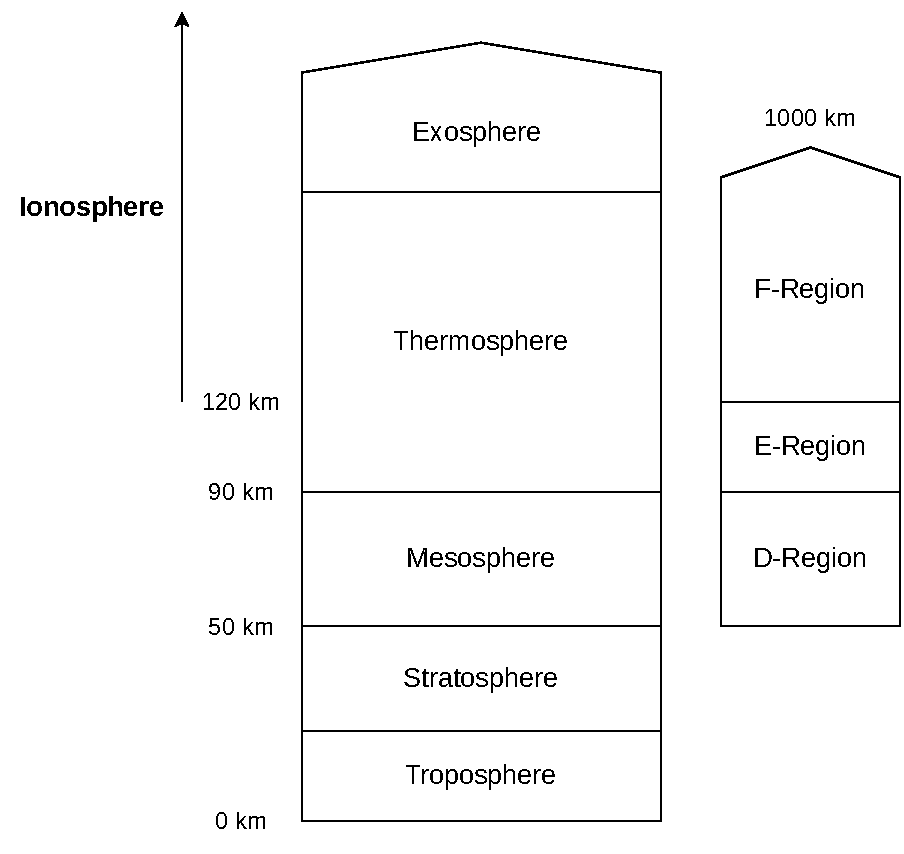
\includegraphics[width=\columnwidth]{figures/atmosphere-model}
                \end{center}
            \end{figure}
        \end{column}
    \end{columns}

\end{frame}

\begin{frame}{Telecommunication Analysis}

    \begin{itemize}
        \item As satellites operate hundreds of kilometers above the Earth's surface, the power of a radio signal transmitted and received by a ground receiver is low
        \vspace{0.3cm}
        \item For the proper functioning of radio communication in a GNSS system, the characteristics of the transmitted signal must be suitable
        \vspace{0.3cm}
        \item The link budget of communication must be performed
    \end{itemize}

\end{frame}

\begin{frame}{Power Budget Analysis}

    \begin{itemize}
        \item Like any space system, the power budget is one of the main aspects to be considered during mission planning
        \vspace{0.1cm}
        \item Considering operational aspects of a GNSS network and the use of small satellites for it, power consumption is a critical aspect
        \vspace{0.1cm}
        \item The power budget of satellite can be determined through three steps:
            \begin{enumerate}
                \item Prepare operating power budget
                \item Size the satellite's battery
                \item Estimate power degradation over mission life
            \end{enumerate}
    \end{itemize}

\end{frame}

\begin{frame}{Orbit Analysis}

    \begin{itemize}
        \item The system's orbit will impact energy aspects, communication, and the lifespan of each satellite in the constellation
        \vspace{0.2cm}
        \item For a global coverage system, more polar orbits (with inclinations closer to 90$^{\circ}$) are preferable
        \vspace{0.2cm}
        \item For regional systems, other types of orbits and elevations can be considered
        \vspace{0.2cm}
        \item Analyses involving orbits can be conducted with the help of simulators using already developed models
    \end{itemize}

\end{frame}
